\documentclass[12pt]{article}
\usepackage[margin=2.4cm, paperwidth=14.8cm, paperheight=21cm]{geometry}
\usepackage{libertine}
\usepackage{xcolor}
\usepackage{tikz}
\usetikzlibrary{decorations.pathmorphing}
\pagestyle{empty}
\setlength{\parindent}{0pt}

\definecolor{gold}{HTML}{8A6D3B}
\definecolor{inknavy}{HTML}{2B3A4A}
\color{inknavy}

% A symmetric calligraphic flourish drawn with Bezier curves.
\newcommand{\flourish}{%
  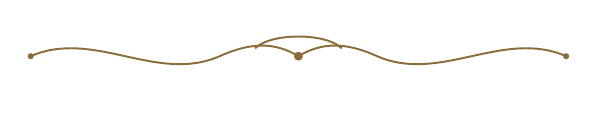
\begin{tikzpicture}[line width=0.7pt, gold]
    \draw (-3.4,0) .. controls (-2.6,0.35) and (-1.8,-0.35) .. (-1.0,0)
      .. controls (-0.6,0.18) and (-0.3,0.18) .. (0,0)
      .. controls (0.3,0.18) and (0.6,0.18) .. (1.0,0)
      .. controls (1.8,-0.35) and (2.6,0.35) .. (3.4,0);
    \fill (0,0) circle (1.6pt);
    \fill (-3.4,0) circle (1.1pt);
    \fill (3.4,0) circle (1.1pt);
    \draw (-0.55,0.10) .. controls (-0.35,0.30) and (0.35,0.30) .. (0.55,0.10);
  \end{tikzpicture}}

% Corner ornament for the frame.
\newcommand{\corner}{%
  \draw[gold, line width=0.7pt]
    (0,0) .. controls (0.5,0.05) and (0.9,0.25) .. (1.1,0.7)
    (0,0) .. controls (0.05,0.5) and (0.25,0.9) .. (0.7,1.1);
  \fill[gold] (0,0) circle (1.5pt);}

\begin{document}

% Full-page double frame with corner ornaments.
\begin{tikzpicture}[remember picture, overlay]
  \draw[gold, line width=1.1pt]
    ([shift={(0.9,0.9)}]current page.south west)
    rectangle ([shift={(-0.9,-0.9)}]current page.north east);
  \draw[gold!60, line width=0.5pt]
    ([shift={(1.12,1.12)}]current page.south west)
    rectangle ([shift={(-1.12,-1.12)}]current page.north east);
  \begin{scope}[shift={([shift={(1.3,1.3)}]current page.south west)}]\corner\end{scope}
  \begin{scope}[shift={([shift={(-1.3,1.3)}]current page.south east)}, xscale=-1]\corner\end{scope}
  \begin{scope}[shift={([shift={(1.3,-1.3)}]current page.north west)}, yscale=-1]\corner\end{scope}
  \begin{scope}[shift={([shift={(-1.3,-1.3)}]current page.north east)}, scale=-1]\corner\end{scope}
\end{tikzpicture}

\begin{center}
\vspace*{0.1cm}
{\color{gold}\itshape Together with their families}

\vspace{0.7cm}
{\fontsize{30}{34}\selectfont\itshape Eleanor Whitfield}

\vspace{0.5cm}
{\color{gold}\large\itshape and}

\vspace{0.5cm}
{\fontsize{30}{34}\selectfont\itshape Marcus Hale}

\vspace{0.55cm}
\flourish

\vspace{0.55cm}
{\large\scshape request the pleasure of your company}\\[0.4em]
{\large\scshape at the celebration of their marriage}

\vspace{0.7cm}
{\color{gold}\Large\scshape Saturday, the twelfth of June}\\[0.5em]
{\color{gold}\large\scshape two thousand and twenty-seven}\\[0.5em]
{\large at four o'clock in the afternoon}

\vspace{0.7cm}
{\Large\itshape Larkspur House and Gardens}\\[0.4em]
{\large 14 Meadowbrook Lane, Ashford Vale}

\vspace{0.7cm}
\flourish

\vspace{0.5cm}
{\small\itshape Dinner and dancing to follow}\\[0.35em]
{\small\itshape Kindly reply by the first of May}
\end{center}

\end{document}
